\begin{tikzpicture}[node distance = 0]
\tikzstyle{every node}=[scale=0.85]
\begin {scope}
\node[draw=white,scale=0.6] (input) at (0,0){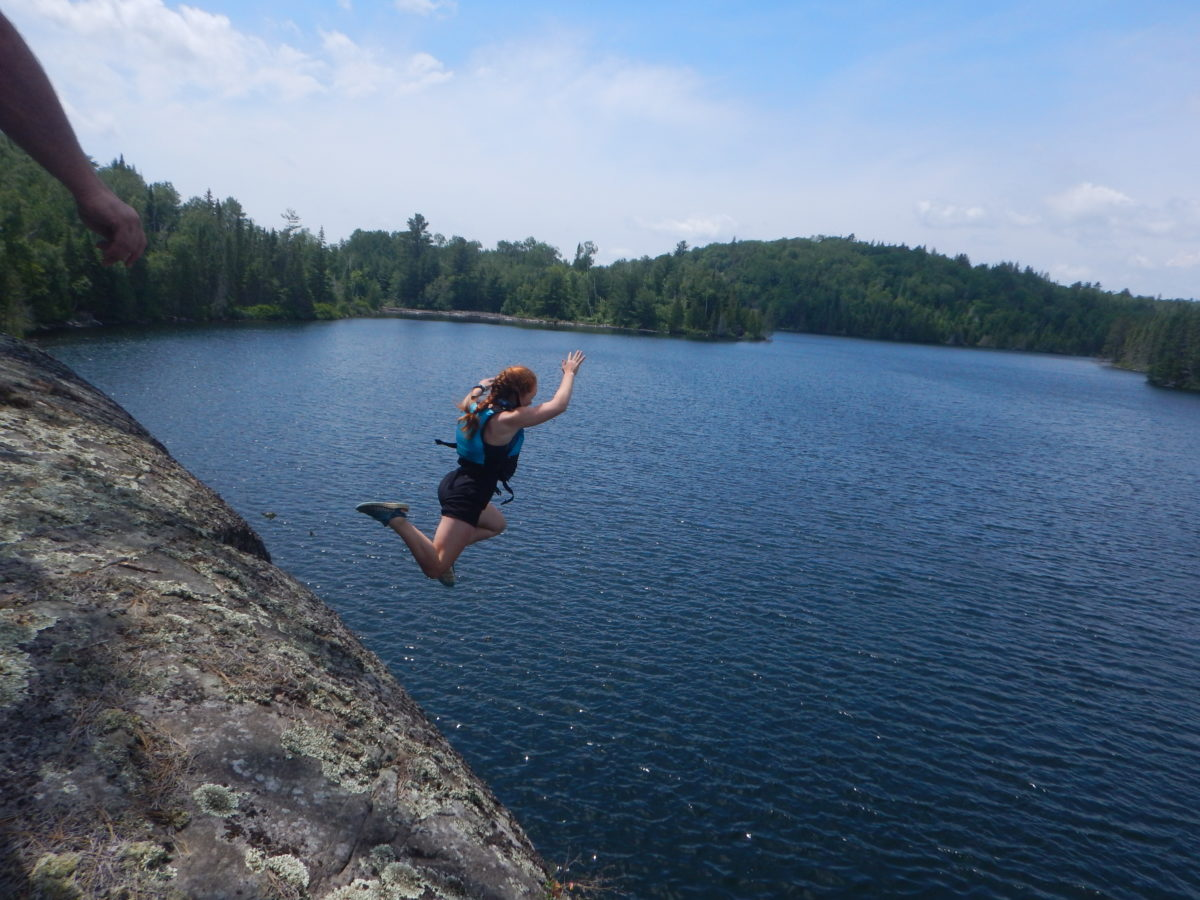
\includegraphics[width=0.62\textwidth]{./Chapter17/Figures/figure-bank-without-attention.jpg}};(1.9,-1.4);
\node[anchor=west] (label1) at ([xshift=-3.5em]input.west) {\begin{tabular}{l}{\normalsize{图片:}}\end{tabular}};
\node[anchor=south] (label2) at ([yshift=-6em]label1.south) {\begin{tabular}{l}{\normalsize{源语言:}}\end{tabular}};
\node[anchor=south] (english1) at ([xshift=-0.28em,yshift=-2.3em]input.south) {\begin{tabular}{l}{\large{A\; girl\; jumps\; off\; a\; {\red{\underline{bank}}}\quad .}}\end{tabular}};

\draw[decorate,decoration={brace,amplitude=4mm},thick] ([xshift=6.3em]input.90) -- ([xshift=0.3em,yshift=-0em]english1.east);

\node[anchor=east,rectangle,thick,rounded corners,minimum width=3.5em,minimum height=2.5em,text centered,draw=black!70,fill=red!25](trans)at ([xshift=7.4em,yshift=5.27em]english1.east){\normalsize{翻译模型}};

\draw[->,thick]([xshift=-1.4em]trans.west) to (trans.west);
\node[anchor=east] (de1) at ([xshift=5.2cm,yshift=-0.1em]trans.east) {\begin{tabular}{l}{\normalsize{目标语言:}}{\normalsize{一个/女孩/从/{\red{河床}}/}}\end{tabular}};
\node[anchor=south] (de2) at ([xshift=1.1em,yshift=-1.5em]de1.south) {\begin{tabular}{l}{\normalsize{上/跳下来/。}} \end{tabular}};
\draw[->,thick](trans.east) to ([xshift=0.5em,yshift=0.1em]de1.west);
\end {scope}
\end{tikzpicture}